\documentclass[UTF8, 12pt, A4paper]{article}



% ---- 导言区 ----
\usepackage{lipsum} % 乱数假文,随机正文用于测试排版效果
\usepackage{xeCJK}  % 中文
\usepackage{fancyhdr} % 页眉页脚
\usepackage[left=2cm, right=2cm, top=2.5cm, bottom=3cm]{geometry} % 页边距
\usepackage{graphicx} % 插入图片
\usepackage{xcolor} % 设置16色字体颜色时需要
\usepackage[colorlinks, linkcolor=blue]{hyperref} % 超链接,可改链接颜色
\usepackage{indentfirst} % 每节首个段落缩进
\usepackage{listings} % 插入代码块
\usepackage{fontspec} % 代码块选字体



% ---- 基本设置区 ----
% 设定页面的页眉页脚类型,$\LaTeX$内置了四种:empty、plain、headings及myheadings,但是我们现在不用这些内置的样式。
\pagestyle{fancy}
% 清除原页眉页脚样式
\fancyhf{} 
% 设置页眉 备注:O代表odd(奇数页),E代表even(偶数页)
\fancyhead[LO, LE]{
    \begin{minipage}[c]{0.06\textwidth}
		
\includegraphics[height=7.5mm]{PMU-SEF-logo.pdf}
	\end{minipage}} % 左页眉
\fancyhead[RO, RE]{右页眉} % 右页眉
% 设置页脚
\fancyfoot[LO, LE]{\textcolor[HTML]{BEBEBE}{\copyright 贝石拌饭}} % 左页脚
% \fancyfoot[RO, RE]{\leftmark} % 右页脚
\fancyfoot[RO, RE]{
    \begin{minipage}[c]{0.06\textwidth}
		
\includegraphics[height=12.5mm]{emergency-food.png}
	\end{minipage}} 
\fancyfoot[CO, CE]{\thepage} % 中页脚
% 页眉线宽,设为0可以去页眉线
\renewcommand{\headrulewidth}{0.2mm} 
% 页脚线宽,设为0可以去页眉线
\renewcommand{\footrulewidth}{0mm} 

% 字体
\setCJKsansfont{Source Han Sans CN} % 思源黑体
% \setCJKmonofont{Sarasa Gothic CL} % 更纱黑体
\setmonofont{Consolas}

% 在section前加入§符号的功能设置(不需要导入包)
\makeatletter
%% See pp. 26f. of 'The LaTeX Companion,' 2nd. ed.
\def\@seccntformat#1{\@ifundefined{#1@cntformat}%
    {\csname the#1\endcsname\quad}%      default
    {\csname #1@cntformat\endcsname}}%   individual control
\newcommand{\section@cntformat}{\S\thesection\quad}
% \newcommand{\subsection@cntformat}{\S\thesubsection\quad}
% \newcommand{\subsubsection@cntformat}{\S\thesubsubsection\quad}
% \newcommand{\paragraph@cntformat}{\S\theparagraph\quad}
% \newcommand{\subparagraph@cntformat}{\S\thesubparagraph\quad}
\makeatletter

% 将作者脚注文本那边的标号也设为特殊符号,不然为数字
\renewcommand{\thefootnote}{\fnsymbol{footnote}}

% 代码块区域设置
\definecolor{mygreen}{rgb}{0,0.6,0}
\definecolor{mygray}{rgb}{0.5,0.5,0.5}
\definecolor{mymauve}{rgb}{0.58,0,0.82}
\lstset{ %
backgroundcolor=\color[RGB]{245,245,244},       % choose the background color
basicstyle=\footnotesize\ttfamily,              % size of fonts used for the code
columns=fullflexible,
breaklines=true,                                % automatic line breaking only at whitespace
captionpos=b,                                   % sets the caption-position to bottom
tabsize=4,
commentstyle=\color{mygreen},                   % comment style
escapeinside={\%*}{*)},                         % if you want to add LaTeX within your code
keywordstyle=\color{blue},                      % keyword style
stringstyle=\color{mymauve}\ttfamily,           % string literal style
frame=single,
rulesepcolor=\color{red!20!green!20!blue!20},
% identifierstyle=\color{red},
language=R,
}



% ---- 封面区 ----
\title{
    
\includegraphics[scale=1]{PMU-logo.pdf} \\ % 封面标题前加图片
    ~\\
    \LaTeX 模板 \\ 案例:凝光怒斥群臣
    }
\author{贝石拌饭\footnotemark[1] \footnotemark[2]}
\date{\today}
\linespread{1.5}



% ---- 正文区 ----
\begin{document}

% 第一页:封面
\maketitle
\footnotetext[1]{Homepage: \url{https://www.zhihu.com/column/CLKuma}} % 作者脚注
\footnotetext[2]{E-Mail: kaede0614@126.com}
\thispagestyle{empty} % 清空封面页的格式

\textbf{说明:}派蒙,最好的应急食品!

% 摘要,可加可不加
% \begin{abstract}
% 本文
% \end{abstract}


% 第二页:目录
\newpage
% 添加目录
\pagenumbering{roman} % 页码数字显示风格
\setcounter{page}{1} % 页码编号手动设置
\tableofcontents

% 正文
\newpage
\setcounter{page}{1}
\pagenumbering{arabic}

% section
\section{section 1}

\begin{figure}[ht]
    \centering
    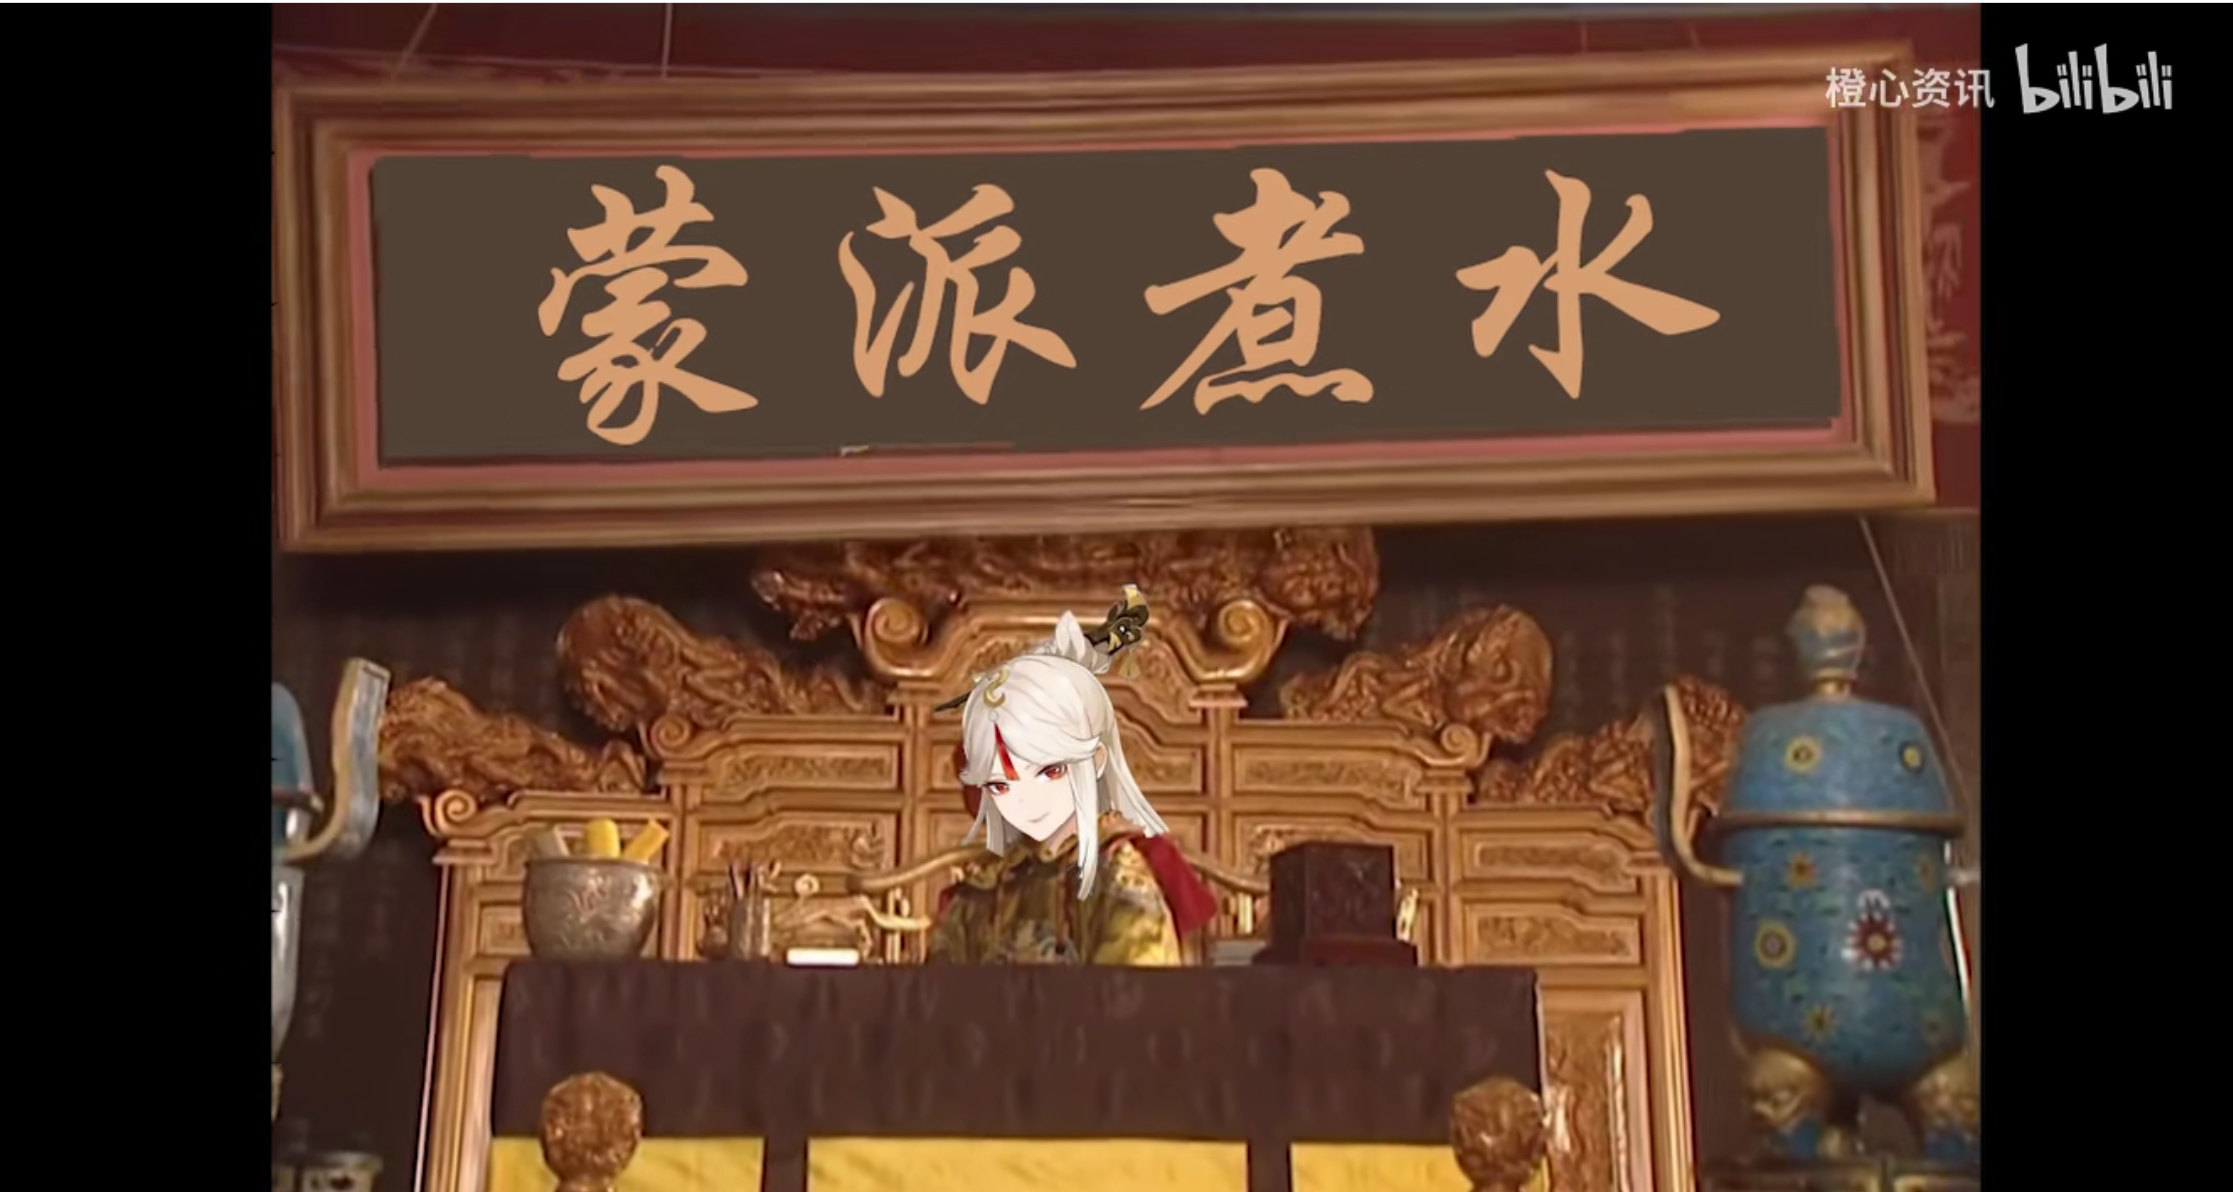
\includegraphics[width=15cm]{蒙派煮水.png}
\end{figure}

前朝护法夜叉统共有五位

朕不得不嫩死四位

璃月七星

朕不得不罢免三位

看看这七个人吧

哪个不是从不出场

哪个不是璃月的栋梁

哪个不是只活在设定里

他们没了,朕心要碎了

帝君把璃月交到朕的手里

却搞成了这个样子

朕是痛心疾首

朕有罪于原神

愧对美工,愧对声乐

朕恨不得

把自己降成四星角色

还有你们

虽然各个冠冕堂皇站在卡池里

你们就真的骗到氪了吗?

朕知道

你们有的人

比这七个人更没用

朕劝你们一句

都把自己的命之座翻出来

晒一晒,洗一洗,拾掇拾掇

朕刚继位的时候

以为璃月最大的敌人是漩涡魔神

灭了漩涡魔神

以为最大的敌人是狗策划

朕 \quad 把狗策划喂了斯大林

螺旋又成了璃月的心头之患

啊,朕改了深渊

蒙德,又成了璃月的心头之患

朕现在是越来越清楚了

璃月的心头之患不在外边

而是在朝廷

就是在这群玉阁!

就在这期的up卡池和常驻当中

咱们这烂一点

米游社就烂一片

你们要是全烂了

臭DD们就会揭竿而起

让我们死无葬身之地啊

想想吧

岩王帝君摩拉克斯

摔死在请仙典仪上才几天呢?

忘了!

那个破烂炉子

还站在玉京台上

天天地盯着你们呢!

朕已经三天三夜没有合眼了

老想着和大伙儿说些什么

可是话,总得有个头啊

想来想去,只有四个字

\begin{figure}[ht]
    \centering
    
\includegraphics[width=10cm]{emergency-food.png}
\end{figure}


\end{document}